\PassOptionsToPackage{unicode=true}{hyperref} % options for packages loaded elsewhere
\PassOptionsToPackage{hyphens}{url}
%
\documentclass[]{article}
\usepackage{lmodern}
\usepackage{amssymb,amsmath}
\usepackage{ifxetex,ifluatex}
\usepackage{fixltx2e} % provides \textsubscript
\ifnum 0\ifxetex 1\fi\ifluatex 1\fi=0 % if pdftex
  \usepackage[T1]{fontenc}
  \usepackage[utf8]{inputenc}
  \usepackage{textcomp} % provides euro and other symbols
\else % if luatex or xelatex
  \usepackage{unicode-math}
  \defaultfontfeatures{Ligatures=TeX,Scale=MatchLowercase}
\fi
% use upquote if available, for straight quotes in verbatim environments
\IfFileExists{upquote.sty}{\usepackage{upquote}}{}
% use microtype if available
\IfFileExists{microtype.sty}{%
\usepackage[]{microtype}
\UseMicrotypeSet[protrusion]{basicmath} % disable protrusion for tt fonts
}{}
\IfFileExists{parskip.sty}{%
\usepackage{parskip}
}{% else
\setlength{\parindent}{0pt}
\setlength{\parskip}{6pt plus 2pt minus 1pt}
}
\usepackage{hyperref}
\hypersetup{
            pdftitle={agro932 - homework1},
            pdfauthor={jinlong},
            pdfborder={0 0 0},
            breaklinks=true}
\urlstyle{same}  % don't use monospace font for urls
\usepackage[margin=1in]{geometry}
\usepackage{color}
\usepackage{fancyvrb}
\newcommand{\VerbBar}{|}
\newcommand{\VERB}{\Verb[commandchars=\\\{\}]}
\DefineVerbatimEnvironment{Highlighting}{Verbatim}{commandchars=\\\{\}}
% Add ',fontsize=\small' for more characters per line
\usepackage{framed}
\definecolor{shadecolor}{RGB}{248,248,248}
\newenvironment{Shaded}{\begin{snugshade}}{\end{snugshade}}
\newcommand{\AlertTok}[1]{\textcolor[rgb]{0.94,0.16,0.16}{#1}}
\newcommand{\AnnotationTok}[1]{\textcolor[rgb]{0.56,0.35,0.01}{\textbf{\textit{#1}}}}
\newcommand{\AttributeTok}[1]{\textcolor[rgb]{0.77,0.63,0.00}{#1}}
\newcommand{\BaseNTok}[1]{\textcolor[rgb]{0.00,0.00,0.81}{#1}}
\newcommand{\BuiltInTok}[1]{#1}
\newcommand{\CharTok}[1]{\textcolor[rgb]{0.31,0.60,0.02}{#1}}
\newcommand{\CommentTok}[1]{\textcolor[rgb]{0.56,0.35,0.01}{\textit{#1}}}
\newcommand{\CommentVarTok}[1]{\textcolor[rgb]{0.56,0.35,0.01}{\textbf{\textit{#1}}}}
\newcommand{\ConstantTok}[1]{\textcolor[rgb]{0.00,0.00,0.00}{#1}}
\newcommand{\ControlFlowTok}[1]{\textcolor[rgb]{0.13,0.29,0.53}{\textbf{#1}}}
\newcommand{\DataTypeTok}[1]{\textcolor[rgb]{0.13,0.29,0.53}{#1}}
\newcommand{\DecValTok}[1]{\textcolor[rgb]{0.00,0.00,0.81}{#1}}
\newcommand{\DocumentationTok}[1]{\textcolor[rgb]{0.56,0.35,0.01}{\textbf{\textit{#1}}}}
\newcommand{\ErrorTok}[1]{\textcolor[rgb]{0.64,0.00,0.00}{\textbf{#1}}}
\newcommand{\ExtensionTok}[1]{#1}
\newcommand{\FloatTok}[1]{\textcolor[rgb]{0.00,0.00,0.81}{#1}}
\newcommand{\FunctionTok}[1]{\textcolor[rgb]{0.00,0.00,0.00}{#1}}
\newcommand{\ImportTok}[1]{#1}
\newcommand{\InformationTok}[1]{\textcolor[rgb]{0.56,0.35,0.01}{\textbf{\textit{#1}}}}
\newcommand{\KeywordTok}[1]{\textcolor[rgb]{0.13,0.29,0.53}{\textbf{#1}}}
\newcommand{\NormalTok}[1]{#1}
\newcommand{\OperatorTok}[1]{\textcolor[rgb]{0.81,0.36,0.00}{\textbf{#1}}}
\newcommand{\OtherTok}[1]{\textcolor[rgb]{0.56,0.35,0.01}{#1}}
\newcommand{\PreprocessorTok}[1]{\textcolor[rgb]{0.56,0.35,0.01}{\textit{#1}}}
\newcommand{\RegionMarkerTok}[1]{#1}
\newcommand{\SpecialCharTok}[1]{\textcolor[rgb]{0.00,0.00,0.00}{#1}}
\newcommand{\SpecialStringTok}[1]{\textcolor[rgb]{0.31,0.60,0.02}{#1}}
\newcommand{\StringTok}[1]{\textcolor[rgb]{0.31,0.60,0.02}{#1}}
\newcommand{\VariableTok}[1]{\textcolor[rgb]{0.00,0.00,0.00}{#1}}
\newcommand{\VerbatimStringTok}[1]{\textcolor[rgb]{0.31,0.60,0.02}{#1}}
\newcommand{\WarningTok}[1]{\textcolor[rgb]{0.56,0.35,0.01}{\textbf{\textit{#1}}}}
\usepackage{graphicx,grffile}
\makeatletter
\def\maxwidth{\ifdim\Gin@nat@width>\linewidth\linewidth\else\Gin@nat@width\fi}
\def\maxheight{\ifdim\Gin@nat@height>\textheight\textheight\else\Gin@nat@height\fi}
\makeatother
% Scale images if necessary, so that they will not overflow the page
% margins by default, and it is still possible to overwrite the defaults
% using explicit options in \includegraphics[width, height, ...]{}
\setkeys{Gin}{width=\maxwidth,height=\maxheight,keepaspectratio}
\setlength{\emergencystretch}{3em}  % prevent overfull lines
\providecommand{\tightlist}{%
  \setlength{\itemsep}{0pt}\setlength{\parskip}{0pt}}
\setcounter{secnumdepth}{0}
% Redefines (sub)paragraphs to behave more like sections
\ifx\paragraph\undefined\else
\let\oldparagraph\paragraph
\renewcommand{\paragraph}[1]{\oldparagraph{#1}\mbox{}}
\fi
\ifx\subparagraph\undefined\else
\let\oldsubparagraph\subparagraph
\renewcommand{\subparagraph}[1]{\oldsubparagraph{#1}\mbox{}}
\fi

% set default figure placement to htbp
\makeatletter
\def\fps@figure{htbp}
\makeatother


\title{agro932 - homework1}
\author{jinlong}
\date{2/19/2020}

\begin{document}
\maketitle

\begin{Shaded}
\begin{Highlighting}[]
\CommentTok{# , include=TRUE, warning=FALSE, echo=TRUE, error=FALSE}
\NormalTok{knitr}\OperatorTok{::}\NormalTok{opts_knit}\OperatorTok{$}\KeywordTok{set}\NormalTok{(}\DataTypeTok{root.dir =} \KeywordTok{normalizePath}\NormalTok{(}\StringTok{'../'}\NormalTok{))}
\NormalTok{knitr}\OperatorTok{::}\NormalTok{opts_chunk}\OperatorTok{$}\KeywordTok{set}\NormalTok{(}\DataTypeTok{warning=}\OtherTok{FALSE}\NormalTok{, }\DataTypeTok{message=}\OtherTok{FALSE}\NormalTok{, }\DataTypeTok{error=}\OtherTok{FALSE}\NormalTok{, }\DataTypeTok{echo=}\OtherTok{TRUE}\NormalTok{)}
\end{Highlighting}
\end{Shaded}

\begin{Shaded}
\begin{Highlighting}[]
\NormalTok{s <-}\StringTok{ }\KeywordTok{scan}\NormalTok{(}\StringTok{'cache/out.sfs'}\NormalTok{)}
\NormalTok{s <-}\StringTok{ }\NormalTok{s[}\OperatorTok{-}\KeywordTok{c}\NormalTok{(}\DecValTok{1}\NormalTok{,}\KeywordTok{length}\NormalTok{(s))]}
\NormalTok{s <-}\StringTok{ }\NormalTok{s}\OperatorTok{/}\KeywordTok{sum}\NormalTok{(s)}
\KeywordTok{barplot}\NormalTok{(s,}\DataTypeTok{names=}\DecValTok{1}\OperatorTok{:}\KeywordTok{length}\NormalTok{(s), }\DataTypeTok{main=}\StringTok{'SFS'}\NormalTok{)}
\end{Highlighting}
\end{Shaded}

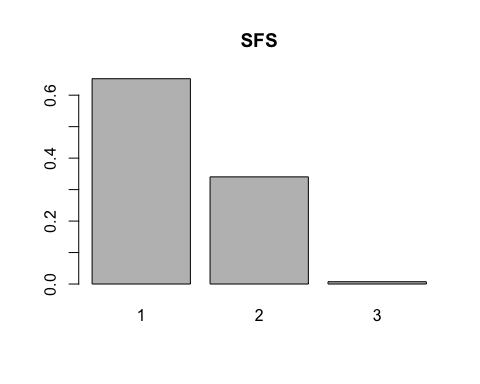
\includegraphics{1.A.1data-simulation_files/figure-latex/unnamed-chunk-1-1.pdf}

\begin{Shaded}
\begin{Highlighting}[]
\NormalTok{t <-}\StringTok{ }\KeywordTok{read.table}\NormalTok{(}\StringTok{"cache/theta.txt"}\NormalTok{)}
\KeywordTok{hist}\NormalTok{(t[,}\DecValTok{4}\NormalTok{])}
\end{Highlighting}
\end{Shaded}

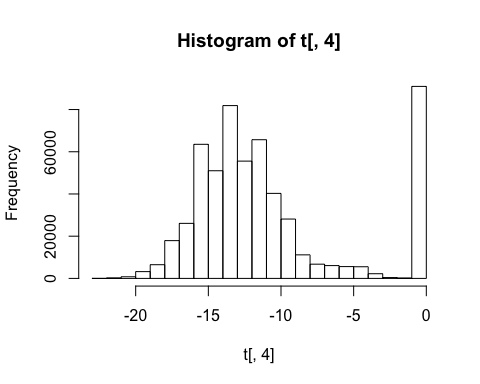
\includegraphics{1.A.1data-simulation_files/figure-latex/unnamed-chunk-1-2.pdf}

\begin{Shaded}
\begin{Highlighting}[]
\NormalTok{fst <-}\StringTok{ }\KeywordTok{read.table}\NormalTok{(}\StringTok{"cache/fst_win.txt"}\NormalTok{, }\DataTypeTok{skip=}\DecValTok{1}\NormalTok{, }\DataTypeTok{header=}\OtherTok{FALSE}\NormalTok{)}
\KeywordTok{names}\NormalTok{(fst)[}\KeywordTok{c}\NormalTok{(}\DecValTok{3}\NormalTok{,}\DecValTok{5}\NormalTok{)] <-}\StringTok{ }\KeywordTok{c}\NormalTok{(}\StringTok{"midp"}\NormalTok{, }\StringTok{"fst"}\NormalTok{)}
\KeywordTok{plot}\NormalTok{(fst}\OperatorTok{$}\NormalTok{midp, fst}\OperatorTok{$}\NormalTok{fst, }\DataTypeTok{xlab=}\StringTok{"Physical position"}\NormalTok{, }\DataTypeTok{ylab=}\StringTok{"Fst"}\NormalTok{, }\DataTypeTok{col=}\StringTok{"#5f9ea0"}\NormalTok{, }\DataTypeTok{pch=}\DecValTok{16}\NormalTok{)}
\end{Highlighting}
\end{Shaded}

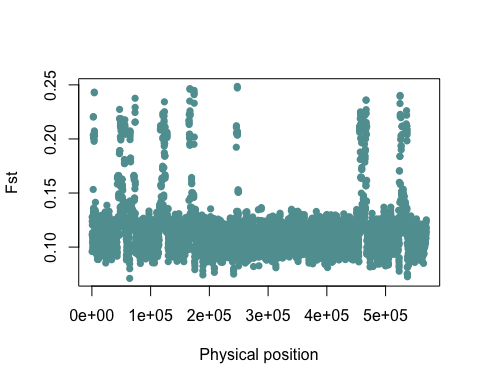
\includegraphics{1.A.1data-simulation_files/figure-latex/unnamed-chunk-1-3.pdf}

\hypertarget{general-feature-format-gff-from-ensemblplants}{%
\section{General feature format (GFF) from
EnsemblPlants}\label{general-feature-format-gff-from-ensemblplants}}

\begin{Shaded}
\begin{Highlighting}[]
\KeywordTok{library}\NormalTok{(}\StringTok{"data.table"}\NormalTok{)}
\CommentTok{## simply read in wouldn't work}
\CommentTok{#gff <- fread("largedata/Zea_mays.B73_RefGen_v4.46.chromosome.Mt.gff3", skip="#", header=FALSE, data.table=FALSE)}
\CommentTok{## grep -v means select lines that not matching any of the specified patterns}
\NormalTok{gff <-}\StringTok{ }\KeywordTok{fread}\NormalTok{(}\DataTypeTok{cmd=}\StringTok{'grep -v "#" largedata/Zea_mays.B73_RefGen_v4.46.chromosome.Mt.gff3'}\NormalTok{, }\DataTypeTok{header=}\OtherTok{FALSE}\NormalTok{, }\DataTypeTok{data.table=}\OtherTok{FALSE}\NormalTok{)}
\CommentTok{#head(gff)}

\KeywordTok{names}\NormalTok{(gff) <-}\StringTok{ }\KeywordTok{c}\NormalTok{(}\StringTok{"seq"}\NormalTok{, }\StringTok{"source"}\NormalTok{, }\StringTok{"feature"}\NormalTok{, }\StringTok{"start"}\NormalTok{, }\StringTok{"end"}\NormalTok{, }\StringTok{"score"}\NormalTok{, }\StringTok{"strand"}\NormalTok{, }\StringTok{"phase"}\NormalTok{, }\StringTok{"att"}\NormalTok{)}
\CommentTok{#table(gff$feature)}
\end{Highlighting}
\end{Shaded}

\hypertarget{get-genes-and-upstream-and-downstream-5kb-regions}{%
\subsubsection{Get genes and upstream and downstream 5kb
regions}\label{get-genes-and-upstream-and-downstream-5kb-regions}}

\begin{Shaded}
\begin{Highlighting}[]
\NormalTok{g <-}\StringTok{ }\KeywordTok{subset}\NormalTok{(gff, feature }\OperatorTok\StringTok{ "gene"}\NormalTok{)}
\NormalTok{g}\OperatorTok{$}\NormalTok{geneid <-}\StringTok{ }\KeywordTok{gsub}\NormalTok{(}\StringTok{".*gene:|;biotype.*"}\NormalTok{, }\StringTok{""}\NormalTok{, g}\OperatorTok{$}\NormalTok{att)}


\CommentTok{### + strand}
\NormalTok{gp <-}\StringTok{ }\KeywordTok{subset}\NormalTok{(g, strand }\OperatorTok\StringTok{ "+"}\NormalTok{) }
\CommentTok{# nrow(gp) 75}

\CommentTok{### get the 5k upstream of the + strand gene model}
\NormalTok{gp_up <-}\StringTok{ }\NormalTok{gp}
\NormalTok{gp_up}\OperatorTok{$}\NormalTok{end <-}\StringTok{ }\NormalTok{gp_up}\OperatorTok{$}\NormalTok{start }\OperatorTok{-}\StringTok{ }\DecValTok{1}
\NormalTok{gp_up}\OperatorTok{$}\NormalTok{start <-}\StringTok{ }\NormalTok{gp_up}\OperatorTok{$}\NormalTok{end }\OperatorTok{-}\StringTok{ }\DecValTok{5000} 

\CommentTok{### get the 5k downstream of the + strand gene model}
\NormalTok{gp_down <-}\StringTok{ }\NormalTok{gp}
\NormalTok{gp_down}\OperatorTok{$}\NormalTok{start <-}\StringTok{ }\NormalTok{gp_down}\OperatorTok{$}\NormalTok{end }\OperatorTok{+}\StringTok{ }\DecValTok{1}
\NormalTok{gp_down}\OperatorTok{$}\NormalTok{end <-}\StringTok{ }\NormalTok{gp_down}\OperatorTok{$}\NormalTok{start }\OperatorTok{+}\StringTok{ }\DecValTok{5000} 
\CommentTok{### - strand}
\NormalTok{gm <-}\StringTok{ }\KeywordTok{subset}\NormalTok{(g, strand }\OperatorTok\StringTok{ "-"}\NormalTok{) }
\CommentTok{# nrow(gm) 82}

\CommentTok{### get the 5k upstream of the + strand gene model}
\NormalTok{gm_up <-}\StringTok{ }\NormalTok{gm}
\NormalTok{gm_up}\OperatorTok{$}\NormalTok{start <-}\StringTok{ }\NormalTok{gm_up}\OperatorTok{$}\NormalTok{end }\OperatorTok{+}\StringTok{ }\DecValTok{1}
\NormalTok{gm_up}\OperatorTok{$}\NormalTok{end <-}\StringTok{ }\NormalTok{gm_up}\OperatorTok{$}\NormalTok{start }\OperatorTok{+}\StringTok{ }\DecValTok{5000} 

\CommentTok{### get the 5k downstream of the + strand gene model}
\NormalTok{gm_down <-}\StringTok{ }\NormalTok{gm}
\NormalTok{gm_down}\OperatorTok{$}\NormalTok{end <-}\StringTok{ }\NormalTok{gm_down}\OperatorTok{$}\NormalTok{start }\OperatorTok{-}\StringTok{ }\DecValTok{1}
\NormalTok{gm_down}\OperatorTok{$}\NormalTok{start <-}\StringTok{ }\NormalTok{gm_down}\OperatorTok{$}\NormalTok{end }\OperatorTok{-}\StringTok{ }\DecValTok{5000} 

\NormalTok{gup <-}\StringTok{ }\KeywordTok{rbind}\NormalTok{(gp_up, gm_up)}
\KeywordTok{fwrite}\NormalTok{(gup, }\StringTok{"cache/mt_gene_up5k.txt"}\NormalTok{, }\DataTypeTok{sep=}\StringTok{"}\CharTok{\textbackslash{}t}\StringTok{"}\NormalTok{, }\DataTypeTok{row.names =} \OtherTok{FALSE}\NormalTok{, }\DataTypeTok{quote=}\OtherTok{FALSE}\NormalTok{)}

\NormalTok{gdown <-}\StringTok{ }\KeywordTok{rbind}\NormalTok{(gp_down, gm_down)}
\KeywordTok{fwrite}\NormalTok{(gdown, }\StringTok{"cache/mt_gene_down5k.txt"}\NormalTok{, }\DataTypeTok{sep=}\StringTok{"}\CharTok{\textbackslash{}t}\StringTok{"}\NormalTok{, }\DataTypeTok{row.names =} \OtherTok{FALSE}\NormalTok{, }\DataTypeTok{quote=}\OtherTok{FALSE}\NormalTok{)}
\end{Highlighting}
\end{Shaded}

\hypertarget{get-genes-and-upstream-and-downstream-5kb-regions-1}{%
\subsection{Get genes and upstream and downstream 5kb
regions}\label{get-genes-and-upstream-and-downstream-5kb-regions-1}}

\begin{Shaded}
\begin{Highlighting}[]
\CommentTok{### - strand}
\NormalTok{gm <-}\StringTok{ }\KeywordTok{subset}\NormalTok{(g, strand }\OperatorTok\StringTok{ "-"}\NormalTok{) }
\KeywordTok{dim}\NormalTok{(gm) }\CommentTok{# 82}
\end{Highlighting}
\end{Shaded}

\begin{verbatim}
## [1] 82 10
\end{verbatim}

\begin{Shaded}
\begin{Highlighting}[]
\KeywordTok{fwrite}\NormalTok{(g, }\StringTok{"cache/mt_gene.txt"}\NormalTok{, }\DataTypeTok{sep=}\StringTok{"}\CharTok{\textbackslash{}t}\StringTok{"}\NormalTok{, }\DataTypeTok{row.names =} \OtherTok{FALSE}\NormalTok{, }\DataTypeTok{quote=}\OtherTok{FALSE}\NormalTok{)}
\end{Highlighting}
\end{Shaded}

\hypertarget{intepret-the-theta-results}{%
\subsection{Intepret the theta
results}\label{intepret-the-theta-results}}

\begin{Shaded}
\begin{Highlighting}[]
\KeywordTok{library}\NormalTok{(}\StringTok{"data.table"}\NormalTok{)}
\KeywordTok{library}\NormalTok{(}\StringTok{"GenomicRanges"}\NormalTok{)}
\KeywordTok{library}\NormalTok{(}\StringTok{"plyr"}\NormalTok{)}
\NormalTok{theta <-}\StringTok{ }\KeywordTok{fread}\NormalTok{(}\StringTok{"cache/theta.txt"}\NormalTok{, }\DataTypeTok{data.table=}\OtherTok{FALSE}\NormalTok{)}
\KeywordTok{names}\NormalTok{(theta)[}\DecValTok{1}\NormalTok{] <-}\StringTok{ "seq"}
\NormalTok{up5k <-}\StringTok{ }\KeywordTok{read.table}\NormalTok{(}\StringTok{"cache/mt_gene_up5k.txt"}\NormalTok{, }\DataTypeTok{header=}\OtherTok{TRUE}\NormalTok{)}
\KeywordTok{names}\NormalTok{(up5k)}
\end{Highlighting}
\end{Shaded}

\begin{verbatim}
##  [1] "seq"     "source"  "feature" "start"   "end"     "score"   "strand" 
##  [8] "phase"   "att"     "geneid"
\end{verbatim}

\begin{Shaded}
\begin{Highlighting}[]
\CommentTok{### define the subject file for theta values}
\NormalTok{grc <-}\StringTok{ }\KeywordTok{with}\NormalTok{(theta, }\KeywordTok{GRanges}\NormalTok{(}\DataTypeTok{seqnames=}\NormalTok{seq, }\KeywordTok{IRanges}\NormalTok{(}\DataTypeTok{start=}\NormalTok{Pos, }\DataTypeTok{end=}\NormalTok{Pos)))}
\CommentTok{### define the query file for genomic feature}
\NormalTok{grf <-}\StringTok{ }\KeywordTok{with}\NormalTok{(up5k, }\KeywordTok{GRanges}\NormalTok{(}\DataTypeTok{seqnames=}\NormalTok{seq, }\KeywordTok{IRanges}\NormalTok{(}\DataTypeTok{start=}\NormalTok{start, }\DataTypeTok{end=}\NormalTok{end), }\DataTypeTok{geneid=}\NormalTok{geneid))}
\CommentTok{### find overlaps between the two}
\NormalTok{tb <-}\StringTok{ }\KeywordTok{findOverlaps}\NormalTok{(}\DataTypeTok{query=}\NormalTok{grf, }\DataTypeTok{subject=}\NormalTok{grc)}
\NormalTok{tb <-}\StringTok{ }\KeywordTok{as.matrix}\NormalTok{(tb)}
\NormalTok{out1 <-}\StringTok{ }\KeywordTok{as.data.frame}\NormalTok{(grf[tb[,}\DecValTok{1}\NormalTok{]])}
\NormalTok{out2 <-}\StringTok{ }\KeywordTok{as.data.frame}\NormalTok{(grc[tb[,}\DecValTok{2}\NormalTok{]])}
\CommentTok{### for each genomic feature, find the sites with non-missing data}
\NormalTok{out <-}\StringTok{ }\KeywordTok{cbind}\NormalTok{(out1, out2[, }\StringTok{"start"}\NormalTok{]) }
\KeywordTok{names}\NormalTok{(out)[}\KeywordTok{ncol}\NormalTok{(out)] <-}\StringTok{ "pos"}
\end{Highlighting}
\end{Shaded}

\hypertarget{intepret-the-theta-results-1}{%
\subsection{Intepret the theta
results}\label{intepret-the-theta-results-1}}

\begin{Shaded}
\begin{Highlighting}[]
\CommentTok{#define unique identifier and merge with the thetas}
\NormalTok{out}\OperatorTok{$}\NormalTok{uid <-}\StringTok{ }\KeywordTok{paste}\NormalTok{(out}\OperatorTok{$}\NormalTok{seqnames, out}\OperatorTok{$}\NormalTok{pos, }\DataTypeTok{sep=}\StringTok{"_"}\NormalTok{)}
\NormalTok{theta}\OperatorTok{$}\NormalTok{uid <-}\StringTok{ }\KeywordTok{paste}\NormalTok{(theta}\OperatorTok{$}\NormalTok{seq, theta}\OperatorTok{$}\NormalTok{Pos, }\DataTypeTok{sep=}\StringTok{"_"}\NormalTok{)}
\NormalTok{df <-}\StringTok{ }\KeywordTok{merge}\NormalTok{(out, theta[, }\KeywordTok{c}\NormalTok{(}\OperatorTok{-}\DecValTok{1}\NormalTok{, }\DecValTok{-2}\NormalTok{)], }\DataTypeTok{by=}\StringTok{"uid"}\NormalTok{)}
\KeywordTok{names}\NormalTok{(theta)}
\end{Highlighting}
\end{Shaded}

\begin{verbatim}
## [1] "seq"            "Pos"            "Watterson"      "Pairwise"      
## [5] "thetaSingleton" "thetaH"         "thetaL"         "uid"
\end{verbatim}

\begin{Shaded}
\begin{Highlighting}[]
\CommentTok{# for each upstream 5k region, how many theta values}
\NormalTok{mx <-}\StringTok{ }\KeywordTok{ddply}\NormalTok{(df, .(geneid), summarise,}
            \DataTypeTok{Pairwise =} \KeywordTok{mean}\NormalTok{(Pairwise, }\DataTypeTok{na.rm=}\OtherTok{TRUE}\NormalTok{),}
            \DataTypeTok{thetaH =} \KeywordTok{mean}\NormalTok{(thetaH, }\DataTypeTok{na.rm=}\OtherTok{TRUE}\NormalTok{),}
            \DataTypeTok{nsites =} \KeywordTok{length}\NormalTok{(uid))}
\end{Highlighting}
\end{Shaded}

\begin{Shaded}
\begin{Highlighting}[]
\NormalTok{get_mean_theta <-}\StringTok{ }\ControlFlowTok{function}\NormalTok{(}\DataTypeTok{gf_file=}\StringTok{"cache/mt_gene_up5k.txt"}\NormalTok{)\{}
  \CommentTok{# gf_file: gene feature file [chr, ="cache/mt_gene_up5k.txt"]}
  
\NormalTok{  theta <-}\StringTok{ }\KeywordTok{fread}\NormalTok{(}\StringTok{"cache/theta.txt"}\NormalTok{, }\DataTypeTok{data.table=}\OtherTok{FALSE}\NormalTok{)}
  \KeywordTok{names}\NormalTok{(theta)[}\DecValTok{1}\NormalTok{] <-}\StringTok{ "seq"}

\NormalTok{  up5k <-}\StringTok{ }\KeywordTok{read.table}\NormalTok{(gf_file, }\DataTypeTok{header=}\OtherTok{TRUE}\NormalTok{)}

  \CommentTok{### define the subject file for theta values}
\NormalTok{  grc <-}\StringTok{ }\KeywordTok{with}\NormalTok{(theta, }\KeywordTok{GRanges}\NormalTok{(}\DataTypeTok{seqnames=}\NormalTok{seq, }\KeywordTok{IRanges}\NormalTok{(}\DataTypeTok{start=}\NormalTok{Pos, }\DataTypeTok{end=}\NormalTok{Pos)))}

  \CommentTok{### define the query file for genomic feature}
\NormalTok{  grf <-}\StringTok{ }\KeywordTok{with}\NormalTok{(up5k, }\KeywordTok{GRanges}\NormalTok{(}\DataTypeTok{seqnames=}\NormalTok{seq, }\KeywordTok{IRanges}\NormalTok{(}\DataTypeTok{start=}\NormalTok{start, }\DataTypeTok{end=}\NormalTok{end), }\DataTypeTok{geneid=}\NormalTok{geneid))}
    
  \CommentTok{### find overlaps between the two}
\NormalTok{  tb <-}\StringTok{ }\KeywordTok{findOverlaps}\NormalTok{(}\DataTypeTok{query=}\NormalTok{grf, }\DataTypeTok{subject=}\NormalTok{grc)}
\NormalTok{  tb <-}\StringTok{ }\KeywordTok{as.matrix}\NormalTok{(tb)}
    
\NormalTok{  out1 <-}\StringTok{ }\KeywordTok{as.data.frame}\NormalTok{(grf[tb[,}\DecValTok{1}\NormalTok{]])}
\NormalTok{  out2 <-}\StringTok{ }\KeywordTok{as.data.frame}\NormalTok{(grc[tb[,}\DecValTok{2}\NormalTok{]])}
  \CommentTok{### for each genomic feature, find the sites with non-missing data}
\NormalTok{  out <-}\StringTok{ }\KeywordTok{cbind}\NormalTok{(out1, out2[, }\StringTok{"start"}\NormalTok{]) }
  \KeywordTok{names}\NormalTok{(out)[}\KeywordTok{ncol}\NormalTok{(out)] <-}\StringTok{ "pos"}

  \CommentTok{#define unique identifier and merge with the thetas}
\NormalTok{  out}\OperatorTok{$}\NormalTok{uid <-}\StringTok{ }\KeywordTok{paste}\NormalTok{(out}\OperatorTok{$}\NormalTok{seqnames, out}\OperatorTok{$}\NormalTok{pos, }\DataTypeTok{sep=}\StringTok{"_"}\NormalTok{)}
\NormalTok{  theta}\OperatorTok{$}\NormalTok{uid <-}\StringTok{ }\KeywordTok{paste}\NormalTok{(theta}\OperatorTok{$}\NormalTok{seq, theta}\OperatorTok{$}\NormalTok{Pos, }\DataTypeTok{sep=}\StringTok{"_"}\NormalTok{)}

\NormalTok{  df <-}\StringTok{ }\KeywordTok{merge}\NormalTok{(out, theta[, }\KeywordTok{c}\NormalTok{(}\OperatorTok{-}\DecValTok{1}\NormalTok{, }\DecValTok{-2}\NormalTok{)], }\DataTypeTok{by=}\StringTok{"uid"}\NormalTok{)}
  \CommentTok{# for each upstream 5k region, how many theta values}

\NormalTok{  mx <-}\StringTok{ }\KeywordTok{ddply}\NormalTok{(df, .(geneid), summarise,}
            \DataTypeTok{Pairwise =} \KeywordTok{mean}\NormalTok{(Pairwise, }\DataTypeTok{na.rm=}\OtherTok{TRUE}\NormalTok{),}
            \DataTypeTok{thetaH =} \KeywordTok{mean}\NormalTok{(thetaH, }\DataTypeTok{na.rm=}\OtherTok{TRUE}\NormalTok{),}
            \DataTypeTok{nsites =} \KeywordTok{length}\NormalTok{(uid))}
  \KeywordTok{return}\NormalTok{(mx)}
\NormalTok{\}}
\end{Highlighting}
\end{Shaded}

\begin{Shaded}
\begin{Highlighting}[]
\CommentTok{### apply the function}
\NormalTok{up5k <-}\StringTok{ }\KeywordTok{get_mean_theta}\NormalTok{(}\DataTypeTok{gf_file=}\StringTok{"cache/mt_gene_up5k.txt"}\NormalTok{)}
\NormalTok{down5k <-}\StringTok{ }\KeywordTok{get_mean_theta}\NormalTok{(}\DataTypeTok{gf_file=}\StringTok{"cache/mt_gene_down5k.txt"}\NormalTok{)}
\KeywordTok{names}\NormalTok{(up5k)}
\end{Highlighting}
\end{Shaded}

\begin{verbatim}
## [1] "geneid"   "Pairwise" "thetaH"   "nsites"
\end{verbatim}

\begin{Shaded}
\begin{Highlighting}[]
\KeywordTok{library}\NormalTok{(}\StringTok{"ggplot2"}\NormalTok{)}
\NormalTok{up5k}\OperatorTok{$}\NormalTok{feature <-}\StringTok{ "up 5k"}
\NormalTok{down5k}\OperatorTok{$}\NormalTok{feature <-}\StringTok{ "down 5k"}
\NormalTok{res <-}\StringTok{ }\KeywordTok{rbind}\NormalTok{(up5k, down5k)}
\KeywordTok{names}\NormalTok{(up5k)}
\end{Highlighting}
\end{Shaded}

\begin{verbatim}
## [1] "geneid"   "Pairwise" "thetaH"   "nsites"   "feature"
\end{verbatim}

\begin{Shaded}
\begin{Highlighting}[]
\KeywordTok{library}\NormalTok{(ggpubr)}
\NormalTok{compaired <-}\StringTok{ }\KeywordTok{list}\NormalTok{(}\KeywordTok{c}\NormalTok{(}\StringTok{"up 5k"}\NormalTok{, }\StringTok{"down 5k"}\NormalTok{) )}

\CommentTok{#res <- as.data.frame(res)}
\KeywordTok{ggplot}\NormalTok{(res, }\KeywordTok{aes}\NormalTok{(}\DataTypeTok{x=}\NormalTok{feature, }\DataTypeTok{y=}\NormalTok{Pairwise, }\DataTypeTok{fill=}\NormalTok{feature)) }\OperatorTok{+}\StringTok{ }
\StringTok{  }\KeywordTok{geom_violin}\NormalTok{(}\DataTypeTok{trim=}\OtherTok{FALSE}\NormalTok{)}\OperatorTok{+}
\StringTok{  }\KeywordTok{labs}\NormalTok{(}\DataTypeTok{title=}\StringTok{"Theta value"}\NormalTok{, }\DataTypeTok{x=}\StringTok{""}\NormalTok{, }\DataTypeTok{y =} \StringTok{"Log10 (theta)"}\NormalTok{)}\OperatorTok{+}
\StringTok{  }\KeywordTok{geom_boxplot}\NormalTok{(}\DataTypeTok{width=}\FloatTok{0.1}\NormalTok{, }\DataTypeTok{fill=}\StringTok{"white"}\NormalTok{)}\OperatorTok{+}
\StringTok{  }\KeywordTok{scale_fill_brewer}\NormalTok{(}\DataTypeTok{palette=}\StringTok{"Blues"}\NormalTok{) }\OperatorTok{+}\StringTok{ }
\StringTok{  }\KeywordTok{geom_signif}\NormalTok{(}\DataTypeTok{comparisons =}\NormalTok{ compaired,}
              \DataTypeTok{step_increase =} \FloatTok{0.1}\NormalTok{,}
              \DataTypeTok{map_signif_level =}\NormalTok{ F,}
              \DataTypeTok{test =}\NormalTok{ t.test)}\OperatorTok{+}
\StringTok{  }\KeywordTok{theme_classic}\NormalTok{()}
\end{Highlighting}
\end{Shaded}

\includegraphics{1.A.1data-simulation_files/figure-latex/unnamed-chunk-9-1.pdf}

\begin{Shaded}
\begin{Highlighting}[]
\KeywordTok{library}\NormalTok{(ggpubr)}
\NormalTok{compaired <-}\StringTok{ }\KeywordTok{list}\NormalTok{(}\KeywordTok{c}\NormalTok{(}\StringTok{"up 5k"}\NormalTok{, }\StringTok{"down 5k"}\NormalTok{)}
\NormalTok{                  )}
\end{Highlighting}
\end{Shaded}

\end{document}
